\documentclass[11pt,letterpaper]{article}
% Shared macros for QVC arXiv v4 (main + TQGL supplement)
% Locked Option A* numbers (fat torus, Tier-C form, frozen-cavity bridge).

\usepackage[utf8]{inputenc}
\usepackage[T1]{fontenc}
\usepackage{amsmath,amssymb,amsthm,mathtools}
\usepackage{graphicx}
\usepackage{caption}
\usepackage{subcaption}
\usepackage{hyperref}
\usepackage{geometry}
\usepackage{float}
\usepackage[section]{placeins}   % FloatBarrier at every \section
\usepackage{tikz}
\usetikzlibrary{arrows.meta,decorations.pathmorphing,positioning,shapes.geometric,calc,3d,fit,backgrounds}
\usepackage{tikz-3dplot}
\usepackage{pgfplots}
\pgfplotsset{compat=1.18}
\usepackage{booktabs}
\usepackage{bm}
\usepackage{xcolor}
\usepackage{enumitem}
\usepackage{array}
\usepackage{multirow}
\usepackage[expansion=false]{microtype}

\geometry{margin=1in}

% Okabe--Ito (colorblind-safe)
\definecolor{oiOrange}{HTML}{E69F00}
\definecolor{oiSky}{HTML}{56B4E9}
\definecolor{oiGreen}{HTML}{009E73}
\definecolor{oiYellow}{HTML}{F0E442}
\definecolor{oiBlue}{HTML}{0072B2}
\definecolor{oiVerm}{HTML}{D55E00}
\definecolor{oiPurple}{HTML}{CC79A7}

\hypersetup{
  colorlinks=true,
  linkcolor=oiBlue,
  citecolor=oiVerm,
  urlcolor=oiBlue,
  pdfauthor={Mineral Hoiland},
  pdftitle={Quantum Vacuum Catalyzation in Topological Excitonic Systems}
}

\newtheorem{theorem}{Theorem}[section]
\newtheorem{lemma}[theorem]{Lemma}
\newtheorem{proposition}[theorem]{Proposition}
\newtheorem{corollary}[theorem]{Corollary}
\newtheorem{definition}[theorem]{Definition}
\newtheorem{remark}[theorem]{Remark}
\newtheorem{hypothesis}{Hypothesis}

\newcommand{\TEVC}{\textsc{TEVC}}
\newcommand{\QVC}{\textsc{QVC}}
\newcommand{\TQGL}{\textsc{TQGL}}
\newcommand{\BKT}{\textsc{BKT}}
\newcommand{\MATBG}{\textsc{MATBG}}
\newcommand{\DCE}{\textsc{DCE}}
\newcommand{\TDVT}{\textsc{TDVT}}
\newcommand{\GPE}{\textsc{GPE}}

\newcommand{\abs}[1]{\left|#1\right|}
\newcommand{\norm}[1]{\left\|#1\right\|}
\newcommand{\dd}[1]{\,\mathrm{d}#1}

% Locked Option A* (fat torus, Tier-C form, frozen-cavity bridge)
\newcommand{\Evac}{0.1287\,\mathrm{meV}}
\newcommand{\Flock}{0.58068}
\newcommand{\elllock}{-2.7958}
\newcommand{\ellcorr}{-2.791}
\newcommand{\alphac}{0.1818}
\newcommand{\Deltac}{0.109\,\mathrm{meV}}
\newcommand{\Deltaex}{0.600\,\mathrm{meV}}
\newcommand{\lfold}{0.8475}
\newcommand{\lstar}{0.7628}
\newcommand{\Deltastar}{0.2324\,\mathrm{meV}}
\newcommand{\hbarcs}{0.07\,\mathrm{meV\cdot\mu m}}
\newcommand{\etaret}{0.137} % a_H evaluation; unique-lock pair is \etaretaH and \etaretph
\newcommand{\etaretaH}{0.137}
\newcommand{\etaretph}{2}
\newcommand{\etaretalt}{3.1}
\newcommand{\xiph}{117\,\mathrm{nm}}
\newcommand{\xialt}{181\,\mathrm{nm}}
\newcommand{\aHlock}{8\,\mathrm{nm}}
\newcommand{\kappaGL}{3.84\times 10^{-5}\,\mathrm{meV\cdot\mu m}^{2}}
\newcommand{\alphaGL}{-0.600\,\mathrm{meV}}
\newcommand{\betaGL}{0.694\,\mathrm{meV}}
\newcommand{\nrefhopf}{0.864}
\newcommand{\alphastar}{0.1636}
\newcommand{\kappaSansatz}{2.46\times 10^{-9}\,\mathrm{meV\cdot\mu m}^{4}}
\newcommand{\Deltacat}{0.502\,\mathrm{meV}}
\newcommand{\gzerofold}{0.109\,\mathrm{meV}}
\newcommand{\pctcat}{16.4\%}
\newcommand{\pctcatfold}{18.2\%}
\newcommand{\hatbarrier}{30\%}
\newcommand{\RwsMatch}{2.18\,\mu\mathrm{m}}
\newcommand{\RwsAlt}{0.91\,\mu\mathrm{m}}
\newcommand{\dsigmaH}{3.87\times 10^{-6}\,\mathrm{S}}
\newcommand{\gzeroeff}{1.365\times 10^{-4}}
\newcommand{\relfroG}{0.0667}
\newcommand{\gzeroeffring}{5.472\times 10^{-4}}
\newcommand{\relfroGring}{0.1564}
\newcommand{\specGws}{\bigl(-1.568,-1.568,-1.162,-1.160,+5.458\bigr)\times 10^{-4}}
\newcommand{\specGring}{\bigl(-7.385,-7.247,-4.326,-2.930,+21.888\bigr)\times 10^{-4}}
\newcommand{\Deltataufive}{0.5720\,\mathrm{meV}}
\newcommand{\gonetaufive}{0.7102}
\newcommand{\Deltatautwenty}{0.6152\,\mathrm{meV}}
\newcommand{\gonetautwenty}{0.8351}
\newcommand{\Deltataufifty}{0.6248\,\mathrm{meV}}
\newcommand{\gonetaufifty}{0.8639}
\newcommand{\Deltanumonly}{0.5697\,\mathrm{meV}}
\newcommand{\gonumonly}{0.8806}
\newcommand{\Deltadephonly}{0.6309\,\mathrm{meV}}
\newcommand{\godephonly}{0.7031}
\newcommand{\Deltafrozencoherent}{0.6623\,\mathrm{meV}}
\newcommand{\gofrozencoherent}{0.1075}
\newcommand{\Deltafrozentaufive}{0.0872\,\mathrm{meV}}
\newcommand{\gofrozentaufive}{0.0102}
\newcommand{\Deltafrozentautwenty}{0.3920\,\mathrm{meV}}
\newcommand{\gofrozentautwenty}{0.0812}
\newcommand{\Deltafrozentaufifty}{0.4761\,\mathrm{meV}}
\newcommand{\gofrozentaufifty}{0.0032}
\newcommand{\gzeroscaled}{0.0527\,\mathrm{meV}}
\newcommand{\lamcat}{0.410}
\newcommand{\redstar}{61.3\%}
\newcommand{\redmax}{81.8\%}
% Coupled GPE / DCE suite (live gap from psi)
\newcommand{\Deltaliveone}{0.6305\,\mathrm{meV}}
\newcommand{\goneps}{0.8832}
\newcommand{\AoneAc}{0.9811}
\newcommand{\AresAc}{0.9117}
\newcommand{\AdetAc}{0.8800}
\newcommand{\Deltassres}{0.2240\,\mathrm{meV}}
\newcommand{\Deltassdet}{0.2461\,\mathrm{meV}}
\newcommand{\gzerostar}{0.0982\,\mathrm{meV}}
\newcommand{\Epair}{0.1963\,\mathrm{meV}}
\newcommand{\Tstar}{118.7\,\mathrm{mK}}
\newcommand{\BerryR}{0.908}
\newcommand{\AcSch}{8.571\,\mu\mathrm{m}^{-1}}
\newcommand{\Acfold}{1.5582\,\mu\mathrm{m}^{-1}}
\newcommand{\gzerohess}{0.0185\,\mathrm{meV}}
\newcommand{\taudark}{662\,\mathrm{ps}}
\newcommand{\taubright}{10.1\,\mathrm{ps}}
\newcommand{\tauratio}{65}
\newcommand{\fluxerr}{3.8\times 10^{-4}}
\newcommand{\Kcanon}{0.407}
\newcommand{\ChernQWZ}{0.993}
\newcommand{\kgeomQWZ}{0.0430\,\mathrm{meV}}
\newcommand{\kgeomfloor}{0.0955\,\mathrm{meV}}
\newcommand{\kconvuv}{0.382\,\mathrm{meV}}
\newcommand{\kappauvtoy}{0.425\,\mathrm{meV}}
\newcommand{\etauv}{0.050}
\newcommand{\etauvsw}{0.053}
\newcommand{\QhopfSthree}{0.9998}
\newcommand{\attachrms}{3.8\times 10^{-16}}
\newcommand{\tlamoverU}{0.379}
\newcommand{\UoverWgap}{0.111}
\newcommand{\KuvTstar}{41.6}
\newcommand{\KfoldTstar}{5.44}
\newcommand{\tlammeV}{0.227\,\mathrm{meV}}
\newcommand{\Wmoire}{5.38\,\mathrm{meV}}
\newcommand{\massdriftcs}{8.3\times 10^{-6}}
\newcommand{\kappafoldtoy}{0.0556\,\mathrm{meV}}
\newcommand{\mstaroverme}{0.99}
\newcommand{\hwphaH}{8.75\,\mathrm{meV}}
\newcommand{\csBog}{1.06\times 10^{5}\,\mathrm{m/s}}
\newcommand{\cLA}{2.14\times 10^{4}\,\mathrm{m/s}}
\newcommand{\nuGPE}{0.290\,\mathrm{THz}}
\newcommand{\omegaGPEps}{1.82\,\mathrm{ps}^{-1}}
\newcommand{\nuStar}{0.112\,\mathrm{THz}}
\newcommand{\qstarLA}{0.0330\,\mathrm{nm}^{-1}}
\newcommand{\lamresLA}{190\,\mathrm{nm}}
\newcommand{\qoverKM}{0.102}
\newcommand{\lamresCS}{0.95\,\mu\mathrm{m}}
\newcommand{\Cvkmin}{0.430\,\mathrm{meV}}
\newcommand{\kappauvfloor}{0.477\,\mathrm{meV}}
\newcommand{\Kuvfloor}{46.7}
\newcommand{\Kfoldfloor}{10.57}
\newcommand{\Fmoire}{1.119}
\newcommand{\Fmoir}{\mathcal{F}_{\text{moir\'{e}}}}
\newcommand{\Ageom}{1.839\,\mu\mathrm{m}^{-1}}
\newcommand{\AgeomF}{2.058\,\mu\mathrm{m}^{-1}}
\newcommand{\lfoldF}{0.7573}
\newcommand{\lstarF}{0.6816}
\newcommand{\DeltaStarF}{0.2914\,\mathrm{meV}}
\newcommand{\GammaschHz}{5.30\times 10^{2}\,\mathrm{Hz}}
\newcommand{\schexp}{19.20}
\newcommand{\qIRpaper}{3.65\times 10^{3}\,\mu\mathrm{m}^{-1}}
\newcommand{\LambdaUV}{125\,\mu\mathrm{m}^{-1}}
\newcommand{\qgapIR}{8.57\,\mu\mathrm{m}^{-1}}

\graphicspath{{figures/}}

% Status tags (use sparingly in running text)
\newcommand{\statusproven}{\textup{\textsc{proven}}}
\newcommand{\statuscomputed}{\textup{\textsc{computed}}}
\newcommand{\statusworking}{\textup{\textsc{frozen working}}}
\newcommand{\statusprogram}{\textup{\textsc{program}}}
\newcommand{\statusconjecture}{\textup{\textsc{conjecture}}}
\newcommand{\statusansatz}{\textup{\textsc{ansatz}}}
\newcommand{\statusmatched}{\textup{\textsc{matched}}}
\newcommand{\statuslocked}{\textup{\textsc{locked}}}
\newcommand{\statusderived}{\textup{\textsc{derived here}}}
\newcommand{\statustruncated}{\textup{\textsc{truncated}}}
\newcommand{\statusdiag}{\textup{\textsc{diagnostic}}}


\title{\textbf{Quantum Vacuum Catalyzation in Topological Excitonic Systems:}\\
\large Frozen-cavity vacuum energy, fold criticality, and parallel catalytic channels}
\author{Mineral Hoiland\\
\textit{Independent Researcher}\\
\href{mailto:mineralhoilandphysics@gmail.com}{mineralhoilandphysics@gmail.com}\\
ORCID: \href{https://orcid.org/0009-0001-2696-644X}{0009-0001-2696-644X}}
\date{8 September 2026}

\begin{document}
\maketitle

\begin{abstract}
We formulate Quantum Vacuum Catalyzation (\QVC) as a catalytic coupling between zero-point fluctuations and an excitonic condensate in Topological Excitonic Vacuum Crystals (\TEVC{}s), exemplified by magic-angle twisted bilayer graphene (\MATBG). Vacuum fluctuations do not supply net energy; they reshape the effective barrier that controls gap formation and defect nucleation. Starting from a phonon-condensate path integral we obtain the locked gap map $\delta=1+\alpha(\ln\delta+\ell)$, which undergoes a saddle-node fold rather than a Berezinskii--Kosterlitz--Thouless essential singularity unless a vortex renormalization group is derived. On the frozen-working fat torus $(r,R)=(8,50)$\,nm with the Tier-C spectral form $E_{\mathrm{vac}}=(1/(4\pi^2))(\hbar c_s/r)F(2\pi r/R)$ and $\hbar c_s=\hbarcs$, the Bessel sum evaluates to $F=\Flock$ and $E_{\mathrm{vac}}=\Evac$, replacing the withdrawn folklore $F=0.596$ and $E_{\mathrm{Cas}}=0.244$\,meV. The derived bridge $\alpha=\lambda E_{\mathrm{vac}}/\Delta_0$ with frozen-cavity logarithm $\ell(r)=\elllock$ (matching the Corrections value $\ell=\ellcorr$ to $0.17\%$) places unit participation past the fold ($\alpha/\alpha_c\approx 1.18$). A physical static gap exists only for $\lambda\le\lambda_{\mathrm{fold}}=\lfold$; the recommended working point $\lambda^\star=\lstar$ yields $\Delta^\star=\Deltastar$ (a $\redstar$ reduction from $\Delta_0=\Deltaex$). The deepest static reduction on the physical branch is $\redmax$ at $\Delta_c=\Deltac$. Catalyzon hybridization through democratic $G=g_0(J-I)$ is a parallel channel with $\lambda_{\min}=-g_0$ (multiplicity $N-1$), not a stacked correction, and the previous $g_0=0.21$\,meV is withdrawn as a vacuum scale. Time-dependent numerics solve a truncated Gross--Pitaevskii equation coupled to a dynamical Casimir amplitude and read the gap from $\psi$. Over $1$\,ps the live gap rises from $\Delta_0$ to $\Deltaliveone$, rather than collapsing; fold-slaved DCE saturates at $A^*/A_c^{\mathrm{fold}}=\AresAc$ (resonant) and $\AdetAc$ (detuned), not $0.52$. Fractional Hall charge $Q_H=1/N$ follows from Chern--Simons invariants and linking on $L(N,1)$, where $H_2=0$. We distinguish proven algebra from computed meV values, program-level $G_{ij}$ and GPE/DCE output, and conjectural spacetime extensions.
\end{abstract}

\begin{figure}[H]
\centering
% Graphical abstract: Option A* pipeline (TikZ, Okabe--Ito)
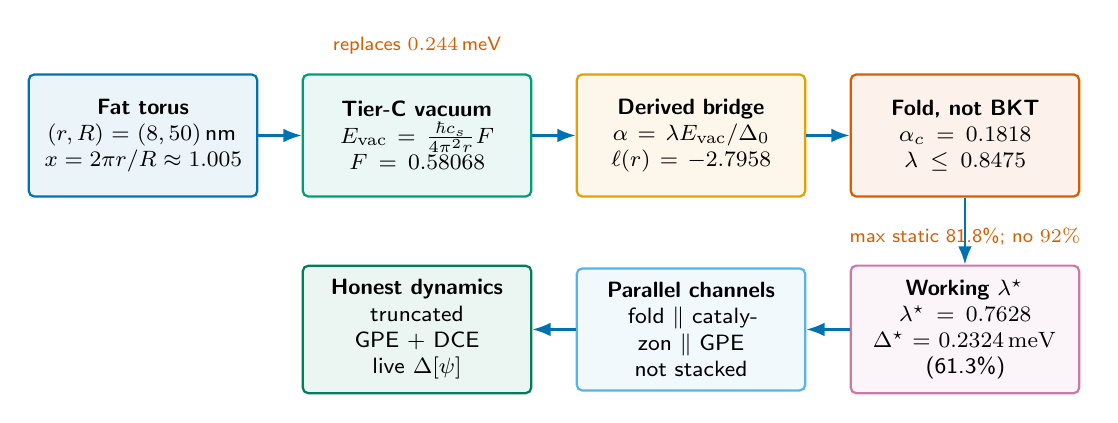
\begin{tikzpicture}[
  font=\sffamily\footnotesize,
  box/.style={draw=#1, line width=0.8pt, rounded corners=2pt,
    fill=#1!8, align=center, inner sep=5pt, text width=2.55cm,
    minimum height=1.55cm},
  arr/.style={-{Latex}, thick, oiBlue}
]
\node[box=oiBlue] (geom) {\textbf{Fat torus}\\$(r,R)=(8,50)$\,nm\\$x=2\pi r/R\approx 1.005$};
\node[box=oiGreen, right=0.55cm of geom] (form) {\textbf{Tier-C vacuum}\\$E_{\mathrm{vac}}=\frac{\hbar c_s}{4\pi^2 r}F$\\$F=\Flock$};
\node[box=oiOrange, right=0.55cm of form] (bridge) {\textbf{Derived bridge}\\$\alpha=\lambda E_{\mathrm{vac}}/\Delta_0$\\$\ell(r)=\elllock$};
\node[box=oiVerm, right=0.55cm of bridge] (fold) {\textbf{Fold, not BKT}\\$\alpha_c=\alphac$\\$\lambda\le\lfold$};
\node[box=oiPurple, below=0.85cm of fold] (star) {\textbf{Working $\lambda^\star$}\\$\lambda^\star=\lstar$\\$\Delta^\star=\Deltastar$ (\redstar)};
\node[box=oiSky, left=0.55cm of star] (par) {\textbf{Parallel channels}\\fold $\parallel$ catalyzon $\parallel$ GPE\\not stacked};
\node[box=oiGreen!80!black, left=0.55cm of par] (hon) {\textbf{Honest dynamics}\\truncated GPE + DCE\\live $\Delta[\psi]$};
\draw[arr] (geom) -- (form);
\draw[arr] (form) -- (bridge);
\draw[arr] (bridge) -- (fold);
\draw[arr] (fold) -- (star);
\draw[arr] (star) -- (par);
\draw[arr] (par) -- (hon);
\node[font=\sffamily\scriptsize, oiVerm, above=0.12cm of form] {replaces $0.244$\,meV};
\node[font=\sffamily\scriptsize, oiVerm, above=0.12cm of star] {max static \redmax; no $92\%$};
\end{tikzpicture}

\caption{\textbf{Graphical abstract.} The working fat-torus geometry and Bessel vacuum form determine the $\alpha$--$E_{\mathrm{vac}}$ bridge and the gap on the physical fold branch at working participation $\lambda^\star$. Fold, catalyzon, and truncated Ginzburg--Landau dynamics are parallel channels.}
\label{fig:graphical}
\end{figure}

\section{Introduction}
\label{sec:intro}

The zero-point energy of a quantized field is a direct consequence of canonical quantization: each mode of frequency $\omega$ contributes $\tfrac12\hbar\omega$ in the ground state. Absolute sums over modes diverge, but differences between boundary configurations are finite and observable, as in the Casimir force between conducting plates~\cite{Casimir1948,Lamoreaux1997}. Quantum Vacuum Catalyzation asks a different question. Can zero-point fluctuations of electromagnetic and phononic fields coherently reshape the effective energy landscape that governs barrier-crossing processes in a strongly correlated condensate, producing measurable consequences in transport, spectroscopy, and pair production, without violating energy conservation?

The proposed answer is catalytic rather than energetic. In every process considered here the energy required to create pairs, nucleate defects, or close a gap is supplied by external drives, chemical potential, or the condensate's own interaction energy. The vacuum plays the role of an enzyme: it changes the topography of the effective potential so that the relevant saddle lies lower, while remaining unconsumed. Rate enhancement is therefore exponential in a reduced barrier, not a claim of net energy extraction from the zero-point sea.

The platform is a Topological Excitonic Vacuum Crystal (\TEVC), realized where a moir\'e superlattice, nontrivial band topology, and broken chirality coexist~\cite{Cao2018correlated,Cao2018unconventional,Andrei2020,Balents2020,Regan2020,Tang2020,Gutierrez2016}. Magic-angle twisted bilayer graphene near $\theta\approx 1.1^\circ$ supplies a moir\'e period $\lambda_M\approx 13$\,nm, flat bands with $W\lesssim 10$\,meV, and a Coulomb scale large enough that $U/W$ is of order ten. In that regime kinetic energy no longer dominates the vacuum correction, yet the geometric scale remains far from the atomic cutoff, so self-consistent feedback between condensate stiffness and cavity amplitude is physically relevant.

A previous preprint generation identified $E_{\mathrm{Cas}}=0.244$\,meV, a static self-consistent gap $\Delta_{\mathrm{QVC}}=0.389$\,meV, and a one-picosecond collapse to $0.032$\,meV quoted as $92\%$. Those numbers are not used as physical results in the present work. The old Casimir formula does not reproduce $0.244$\,meV on the stated geometry; the three percentages mixed distinct mechanisms and distinct baselines; and the dynamical solver that produced $0.032$\,meV prescribed $\Delta(t)$ independently of the condensate field $\psi$. The present manuscript freezes Option~A*: the fat torus $(r,R)=(8,50)$\,nm, the Tier-C spectral form, package $\hbar c_s=\hbarcs$, and the derived bridge from $E_{\mathrm{vac}}$ into the locked fold map. On that triple one finds $F=\Flock$ and $E_{\mathrm{vac}}=\Evac$. Unit participation is past the fold. Working physics, if any remains gapped, lives at $\lambda\le\lambda_{\mathrm{fold}}=\lfold$, with recommended $\lambda^\star=\lstar$ and $\Delta^\star=\Deltastar$.

Section~\ref{sec:tevc} defines the \TEVC{} and the symmetry-breaking cascade. Section~\ref{sec:gap} derives the gap map and the fold theorem. Section~\ref{sec:vacuum} evaluates the toroidal vacuum energy. Section~\ref{sec:bridge} constructs the $\alpha$--$E_{\mathrm{vac}}$ bridge. Section~\ref{sec:lambda} introduces participation $\lambda$ and forbids stacking of parallel channels. Section~\ref{sec:catalyzon} treats democratic $\mathrm{Spec}(G)$ and the program-level Wigner--Seitz matrix $G_{ij}$. Section~\ref{sec:tqgl} states the topological Ginzburg--Landau functional and the truncated equations actually intended for numerics. Section~\ref{sec:hopf} derives $Q_H=1/N$. Section~\ref{sec:experiments} lists experimental signatures. Section~\ref{sec:status} records epistemic status. Appendices collect the fold table and the withdrawn folklore.

\section{The \TEVC{} platform}
\label{sec:tevc}

\begin{definition}[Topochirality]
A crystal is topochiral if it simultaneously supports (i)~a moir\'e superlattice with period $\lambda_M\gg a_{\mathrm{atomic}}$, furnishing a Casimir cavity at the geometric scale of the condensate; (ii)~nontrivial band topology, with Berry curvature $\Omega(\mathbf{k})$ and Chern number $C\neq 0$; and (iii)~broken time-reversal or sublattice (chirality) symmetry, induced by Kekul\'e bond order or spin--orbit coupling, that selects a definite handedness for hopfion textures.
\end{definition}

No single property is sufficient. The superlattice sets the cavity; topology underwrites a quantized Hall response; broken chirality selects hopfion handedness. For \MATBG{} two graphene sheets twisted by $\theta\approx 1.1^\circ$ produce $\lambda_M=a/[2\sin(\theta/2)]\approx 13$\,nm and a pair of nearly flat moir\'e bands~\cite{Cao2018correlated,Cao2018unconventional,Andrei2020,Balents2020}. Analogous physics appears in transition-metal dichalcogenide heterobilayers~\cite{Regan2020,Tang2020}.

The \TEVC{} ground state is reached by a cascade rather than a single mean-field transition. Starting from the enlarged $U(4)\times U(4)$ symmetry of the flat-band manifold (spin $\otimes$ valley), valley polarization at $T_1\sim 30$\,K and Kekul\'e order at $T_2\sim 6$\,K act as a trilinear source
\begin{equation}
\mathcal{F}_{\mathrm{tri}}=\delta\,\Delta_{\mathrm{ex}}^*\Delta_{KK'}P_v+\mathrm{h.c.}
\end{equation}
for the excitonic order parameter, so that condensation at $T_{\mathrm{BEC}}\sim 1$\,K is inductive. Once the condensate stiffens, its toroidal cavity reaches the aspect ratio of the freeze, and vacuum coupling enters non-thermally.

Three energy scales interact. The exchange $J\sim 0.3$\,meV sets the bare excitonic gap $\Delta_0=2J=\Deltaex$. The phononic scale $\hbar\omega_{\mathrm{ph}}\sim\hbar c_s/a_H$ is tens of microelectronvolts for $a_H\sim 8$\,nm. The vacuum energy $E_{\mathrm{vac}}(r,R)$ of a toroidal core with minor radius $r\sim a_H$ and major radius $R\sim\xi$ determines the zero-point amplitude that feeds the gap map. The vacuum correction is neither a negligible perturbation (flat bands quench the kinetic energy that would otherwise dominate) nor a leading atomic-scale Casimir force (the moir\'e period remains well separated from the carbon lattice). It occupies the intermediate window in which self-consistent feedback is interesting.

\section{Self-consistent gap equation and fold theorem}
\label{sec:gap}

The Euclidean action of an excitonic condensate $\Psi$ coupled linearly to a phonon field $\phi$ is $S=S_\Psi+S_\phi+S_{\Psi\phi}$, with
\begin{align}
S_\Psi&=\int\mathrm{d}\tau\,\mathrm{d}^2r\Bigl[\Psi^*\partial_\tau\Psi+\frac{\hbar^2}{2m^*}|\nabla\Psi|^2+\alpha|\Psi|^2+\frac{\beta}{2}|\Psi|^4\Bigr],\\
S_\phi&=\frac12\int\mathrm{d}\tau\,\mathrm{d}^2r\bigl[(\partial_\tau\phi)^2+(c_s\nabla\phi)^2\bigr],\\
S_{\Psi\phi}&=g\int\mathrm{d}\tau\,\mathrm{d}^2r\,\phi\,|\Psi|^2.
\end{align}
Because $S_\phi$ is quadratic, the phonon may be integrated exactly. The resulting retarded kernel is $D(\mathbf{q},\omega_n)=1/(\omega_n^2+c_s^2 q^2)$. Retardation is controlled by
\begin{equation}
\eta_{\mathrm{ret}}=\frac{2\Delta_0\xi}{\hbar c_s}.
\end{equation}
With the causal-propagator identification of $\xi$ used in the original derivation one obtains $\eta_{\mathrm{ret}}\approx\etaret$, above the marginality threshold $\sim 2$, so that a static decoupling is consistent to relative order $1/\eta_{\mathrm{ret}}^2$. (Identifying $\xi$ with the fat-torus major radius $R=50$\,nm would give a different numerical value; we retain $\eta_{\mathrm{ret}}\approx\etaret$ as the locked causal-propagator figure and do not promote it to a derived duality.)

After BCS-like decoupling, a Matsubara sum over a logarithmically diverging flat-band density of states, ultraviolet regularization at the healing length, and analytic continuation, the self-consistent gap including a dimensionless zero-point amplitude $A$ reads
\begin{equation}
\Delta=\Delta_0+\hbar c_s A\Bigl[\ln\frac{\Delta a_H}{2\hbar c_s}+\gamma_E\Bigr],
\label{eq:gap}
\end{equation}
with $\Delta_0=2J$ and $\gamma_E$ the Euler--Mascheroni constant. Frozen-cavity geometry sets $a_H=r=\mathrm{const}$. Dimensionless variables $\delta=\Delta/\Delta_0$,
\begin{equation}
\ell(r)=\ln\frac{\Delta_0 r}{2\hbar c_s}+\gamma_E,\qquad
\alpha=\frac{\hbar c_s A}{\Delta_0}
\end{equation}
convert Eq.~\eqref{eq:gap} into the locked map
\begin{equation}
\delta=1+\alpha(\ln\delta+\ell).
\label{eq:foldmap}
\end{equation}

\begin{theorem}[Saddle-node fold]
\label{thm:fold}
For $\ell<\ln\delta$ on the physical branch, Eq.~\eqref{eq:foldmap} admits a saddle-node (fold) bifurcation at $\alpha_c=\delta_c$ with
\begin{equation}
\delta_c\bigl(1-\ln\delta_c-\ell\bigr)=1.
\end{equation}
Near the fold, $\delta-\delta_c\sim\pm\sqrt{\alpha_c-\alpha}$. There is no real gapped solution for $\alpha>\alpha_c$. A Berezinskii--Kosterlitz--Thouless essential singularity $\Delta\sim\exp(-C/\sqrt{A_c-A})$~\cite{Berezinskii1971,Kosterlitz1973} would require vortex proliferation in $\arg\Psi$ and is contingent on a vortex renormalization group that is not derived here.
\end{theorem}

On the frozen cavity one finds $\ell(r)=\elllock$ versus the Corrections value $\ell=\ellcorr$ (relative error $0.17\%$). The Corrections logarithm is this frozen-cavity logarithm, not an independent infrared fit. The corresponding critical point is $\alpha_c=\delta_c=\alphac$, hence $\Delta_c=\delta_c\Delta_0=\Deltac$. Running healing $a_H=\hbar c_s/\Delta$ produces instead $\ell_{\mathrm{tree}}=\ln\tfrac12+\gamma_E\approx-0.116$ and an exponentially small $F$ when $a_H\gg R$; that is a different theory and is not used as the freeze.

The physical content is catalytic. The effective Landau coefficient acquires a logarithm in $|\Psi|$, so the saddle between the condensed vacuum and the competing symmetric state is pulled toward the condensate manifold as $A$ increases, until the two branches merge and disappear. Experimental discrimination between square-root fold softening and an essential singularity remains a sharp test (hypothesis H-VRG1).

\begin{figure}[H]
\centering
% Saddle-node fold from locked solver data
\begin{tikzpicture}
\begin{axis}[
  width=0.92\linewidth,
  height=6.2cm,
  xlabel={$\alpha/\alpha_c$},
  ylabel={$\delta=\Delta/\Delta_0$},
  xmin=0, xmax=1.05,
  ymin=0, ymax=1.08,
  legend style={draw=none, at={(0.02,0.02)}, anchor=south west, font=\footnotesize, cells={anchor=west}},
  tick label style={font=\small},
  label style={font=\small},
  clip=false,
]
\addplot[oiBlue, thick, forget plot]
  table[x index=0, y index=2, skip first n=1] {data/fold_phys.dat};
\addlegendimage{oiBlue, thick}
\addlegendentry{physical $\delta_+$}
\addplot[oiVerm, thick, dashed, forget plot]
  table[x index=0, y index=2, skip first n=1] {data/fold_unst.dat};
\addlegendimage{oiVerm, thick, dashed}
\addlegendentry{unstable $\delta_-$}
\addplot[only marks, mark=*, mark size=2.4pt, oiVerm]
  coordinates {(1.0, 0.1818)};
\addlegendentry{fold $(\alpha_c,\delta_c)$}
\addplot[only marks, mark=square*, mark size=2.4pt, oiOrange]
  coordinates {(0.90, 0.3874)};
\addlegendentry{$\lambda^\star$ ($\alpha/\alpha_c=0.90$)}
\draw[oiGreen, densely dotted] (axis cs:0,0.1818) -- (axis cs:1.0,0.1818);
\end{axis}
\end{tikzpicture}

\caption{\textbf{Locked fold of the gap map.} Physical and unstable branches of $\delta=1+\alpha(\ln\delta+\ell)$ at $\ell=\elllock$, computed by the fold solver (data file \texttt{fold\_phys.dat}, \texttt{fold\_unst.dat}). The branches merge at $\alpha_c=\delta_c=\alphac$. The square marks the working point $\lambda^\star$ with $\alpha/\alpha_c=0.90$. Square-root scaling holds near the fold; BKT phenomenology is not included.}
\label{fig:fold}
\end{figure}

\section{Toroidal vacuum energy (Option A*)}
\label{sec:vacuum}

Each hopfion in the \TEVC{} presents a toroidal cavity of minor radius $r\sim a_H$ and major radius $R\sim\xi$ (Fig.~\ref{fig:torus}). The locked spectral form (Tier~C, two-dimensional phase-space measure) is
\begin{equation}
E_{\mathrm{vac}}=\frac{1}{4\pi^2}\frac{\hbar c_s}{r}\,F\!\left(\frac{2\pi r}{R}\right),\qquad
F(x)=\sum_{n=1}^\infty K_0(nx),
\label{eq:tierc}
\end{equation}
with $K_0$ the modified Bessel function of the second kind. The proximity-force approximation is uncontrolled in the fat-torus regime $x\sim 1$. Mode quadrature $A_{\mathrm{eff}}=\sqrt{n}\,A_{\mathrm{single}}$ is a distinct channel: $F$ already sums toroidal windings, and $\sqrt{n}$ is not inserted into the static gap loop.

\begin{figure}[H]
\centering
% Fat-torus Casimir cavity (schematic)
\tdplotsetmaincoords{70}{115}
\begin{tikzpicture}[tdplot_main_coords, scale=1.15]
\pgfmathsetmacro{\R}{2.15}
\pgfmathsetmacro{\rr}{0.55}
% torus meridians
\foreach \t in {0,20,...,340}{
  \draw[oiBlue!35, thin]
    plot[domain=0:360, samples=36, variable=\u]
    ({\R*cos(\t)+\rr*cos(\t)*cos(\u)}, {\R*sin(\t)+\rr*sin(\t)*cos(\u)}, {\rr*sin(\u)});
}
\draw[oiVerm, very thick] (0,0,0) circle (\R);
\draw[oiGreen, thick] ({\R},0,0) circle ({\rr});
\draw[<->, oiVerm, thick] (0,0,-1.55) -- (\R,0,-1.55)
  node[midway, below, font=\small] {$R=50$\,nm};
\draw[<->, oiGreen, thick] ({\R},0,0) -- ({\R+\rr},0,0)
  node[midway, above, font=\scriptsize, xshift=4pt] {$r=8$\,nm};
\node[font=\small, oiBlue] at (0,0,1.35) {$x=2\pi r/R\approx 1.005$};
\node[font=\small] at (0,-2.9,0) {frozen working geometry (Option A*)};
\node[font=\small, oiVerm] at (2.8,0.2,1.0) {$Q_H=1/N$};
\end{tikzpicture}

\caption{\textbf{Frozen-working fat torus.} Minor radius $r=8$\,nm (healing length) and major radius $R=50$\,nm (coherence geometry) give $x=2\pi r/R\approx 1.005$. This is the Option~A* cavity. The Hopf charge $Q_H=1/N$ is carried by the layered texture, not by a fundamental $2$-cycle of $L(N,1)$.}
\label{fig:torus}
\end{figure}

The old Casimir formula $E_{\mathrm{old}}=(1/4\pi)(\hbar c_s/r)(R/r)F$ evaluates to $2.527$\,meV on the same geometry and therefore does \emph{not} reproduce the preprint claim $0.244$\,meV. That audit is a pass of a negative claim: $0.244$\,meV is not an output of the stated operator on the stated torus. Jacobi $\vartheta_3$ at the moir\'e aspect is numerically unrelated to $F(x)$ and is withdrawn as an identification.

\begin{figure}[H]
\centering
% Toroidal Bessel mode sum F(x)
\begin{tikzpicture}
\begin{axis}[
  width=0.92\linewidth,
  height=6.0cm,
  xlabel={$x=2\pi r/R$},
  ylabel={$F(x)=\sum_{n=1}^{\infty} K_0(nx)$},
  xmin=0.15, xmax=2.4,
  ymin=0, ymax=4.2,
  legend style={draw=none, at={(0.98,0.98)}, anchor=north east, font=\footnotesize},
  tick label style={font=\small},
  label style={font=\small},
]
\addplot[oiBlue, thick]
  table[x index=0, y index=1, skip first n=1] {data/F_bessel.dat};
\addlegendentry{$F(x)$ (Bessel)}
\addplot[oiVerm, densely dashed]
  coordinates {(1.0053,0) (1.0053,4.2)};
\addlegendentry{fat torus $x\approx 1.005$}
\addplot[only marks, mark=*, mark size=2.6pt, oiVerm]
  coordinates {(1.0053, 0.58068)};
\addlegendentry{$F=\Flock$ (not $0.596$)}
\end{axis}
\end{tikzpicture}

\caption{\textbf{Bessel mode sum.} $F(x)=\sum_n K_0(nx)$ on the fat-torus scan. At $x\approx 1.005$ one has $F=\Flock$, replacing the withdrawn $F=0.596$. The $n=1$ truncation $K_0(x)$ errs by $\sim 28\%$ in this regime, so the full sum is required.}
\label{fig:Fbessel}
\end{figure}

Option~A* therefore freezes Eq.~\eqref{eq:tierc} on $(r,R)=(8,50)$\,nm with $\hbar c_s=\hbarcs$. The evaluation is
\begin{equation}
F=\Flock,\qquad E_{\mathrm{vac}}=\Evac.
\end{equation}
The geometric amplitude is $A=E_{\mathrm{vac}}/(\hbar c_s)$, or $AR\approx 0.0919$, replacing the withdrawn $A\xi=0.296$. The meV figure is \emph{computed} from the frozen triple. It is not promoted to a measured \MATBG{} spectroscopic energy, and $\hbar c_s$ remains a platform scale.

The Corrections moir\'e geometry $(r,R)=(0.335,13.4)$\,nm produces $F\approx 8.10$ and an $E_{\mathrm{vac}}$ far past the fold; it is not the freeze. Retuning $\hbar c_s$ to force $0.244$\,meV is likewise refused.

\section{Derived \texorpdfstring{$\alpha$--$E_{\mathrm{vac}}$}{alpha--E\_vac} bridge}
\label{sec:bridge}

At unit participation the condensate sees the full geometric amplitude. Combining the identifications $A=E_{\mathrm{vac}}/(\hbar c_s)$ and $\alpha=\hbar c_s A/\Delta_0$ yields the boxed bridge
\begin{equation}
\alpha=\lambda\frac{E_{\mathrm{vac}}}{\Delta_0}.
\label{eq:bridge}
\end{equation}
Equation~\eqref{eq:bridge} is proven algebra once $\lambda$ is defined as the overlap of the condensate with the cavity mode. It is not an extra fit.

\begin{theorem}[Fold-out at unit participation]
\label{thm:foldout}
On the Option~A* triple, $\lambda=1$ gives $\alpha=E_{\mathrm{vac}}/\Delta_0\approx 0.2145$ and $\alpha/\alpha_c\approx 1.180>1$. The physical branch of Eq.~\eqref{eq:foldmap} does not exist. Absence of a static $\Delta^*$ at unit participation is a theorem of the fold, not a solver failure.
\end{theorem}

The vacuum energy that would recover the withdrawn $35\%$ reduction ($\Delta=0.389$\,meV) is $E\approx 0.065$\,meV, which is neither $0.244$\,meV nor $\Evac$. Package $\hbar c_s$ at the fold (for $\lambda=1$) would be $\approx 0.0593$\,meV$\cdot\mu$m; we do not retune it. Remaining gapped physics at these parameters, if any, is therefore not the static unit-participation vacuum loop. It may live at $\lambda<1$, in the catalyzon channel, or in dynamics.

\section{Participation \texorpdfstring{$\lambda$}{lambda} and parallel channels}
\label{sec:lambda}

The fold bound is immediate from Eq.~\eqref{eq:bridge}:
\begin{equation}
\lambda_{\mathrm{fold}}=\frac{\alpha_c\Delta_0}{E_{\mathrm{vac}}}=\lfold.
\end{equation}
The physical branch exists only for $\lambda\le\lambda_{\mathrm{fold}}$. Its deepest gap is $\Delta_c=\Deltac$, a maximum static reduction of $\redmax$. Consequently $\delta=0.032/0.6\approx 0.053<\delta_c$ cannot be a static physical solution for any $\lambda$. The withdrawn $92\%$ figure is either the unstable branch or a dynamical overshoot of a simulation that used $0.244$\,meV as a drive and ignored $\psi$.

The recommended working point is a conservative fraction of the fold,
\begin{equation}
\lambda^\star=0.90\,\lambda_{\mathrm{fold}}=\lstar,
\end{equation}
at which $\alpha/\alpha_c=0.90$ and the physical root is $\Delta^\star=\Deltastar$ ($\redstar$ reduction). Figure~\ref{fig:lambda} shows the scan.

\begin{figure}[H]
\centering
% Participation scan on the physical fold branch
\begin{tikzpicture}
\begin{axis}[
  width=0.92\linewidth,
  height=6.2cm,
  xlabel={participation $\lambda$},
  ylabel={$\Delta(\lambda)$ (meV)},
  xmin=0.02, xmax=0.90,
  ymin=0.08, ymax=0.62,
  legend style={draw=none, at={(0.02,0.02)}, anchor=south west, font=\footnotesize},
  tick label style={font=\small},
  label style={font=\small},
]
\addplot[oiBlue, thick]
  table[x index=0, y index=3, skip first n=1] {data/lambda_scan.dat};
\addlegendentry{physical branch}
\addplot[oiOrange, densely dashed]
  coordinates {(\lstar,0.08) (\lstar,0.62)};
\addlegendentry{$\lambda^\star=\lstar$}
\addplot[oiVerm, densely dashed]
  coordinates {(\lfold,0.08) (\lfold,0.62)};
\addlegendentry{$\lambda_{\mathrm{fold}}=\lfold$}
\addplot[only marks, mark=square*, mark size=2.5pt, oiOrange]
  coordinates {(\lstar, 0.232)};
\addplot[oiGreen, densely dotted]
  coordinates {(0.02,0.109) (0.90,0.109)};
\node[font=\scriptsize, oiGreen!50!black, anchor=west] at (axis cs:0.04,0.125) {$\Delta_c=\Deltac$ (max static \redmax)};
\end{axis}
\end{tikzpicture}

\caption{\textbf{Gap versus participation.} Physical-branch $\Delta(\lambda)$ from \texttt{lambda\_scan.dat}. Vertical lines mark $\lambda^\star=\lstar$ and $\lambda_{\mathrm{fold}}=\lfold$. The dotted line is $\Delta_c$. There is no physical point with a $92\%$ static reduction.}
\label{fig:lambda}
\end{figure}

Catalyzon hybridization is a second, parallel channel. If the same vacuum feeds off-diagonal mode mixing, $g_0=\lambda_G E_{\mathrm{vac}}$ and $\Delta_{\mathrm{cat}}=\Delta_{\mathrm{ex}}-g_0$. At $\lambda_{\mathrm{fold}}$ one would have $g_0=\Delta_c$ and an $18\%$ catalyzon reduction, not $52\%$. The historical $52\%$ mixed $\Delta_{\mathrm{QVC}}$ with a $0.1$\,meV guess against $\Delta_{\mathrm{ex}}$. Scaling that guess with $E_{\mathrm{vac}}/0.244$ produces $g_0\approx\gzeroscaled$ and $\lambda_{\mathrm{cat}}\approx\lamcat$. The working value $g_0=0.21$\,meV exceeds $E_{\mathrm{vac}}$ and is withdrawn as a vacuum scale.

Unitarity of participation reads $\lambda_\alpha+\lambda_G\le 1$. An equal split $(0.5,0.5)$ is subcritical on both channels. Fold, catalyzon, and time-dependent Ginzburg--Landau evolution must be reported in parallel (Fig.~\ref{fig:channels}). Adding $35\%+52\%+92\%$ is meaningless: the percentages used different baselines and, in the third case, a prescribed gap.

\begin{figure}[H]
\centering
% Parallel channels
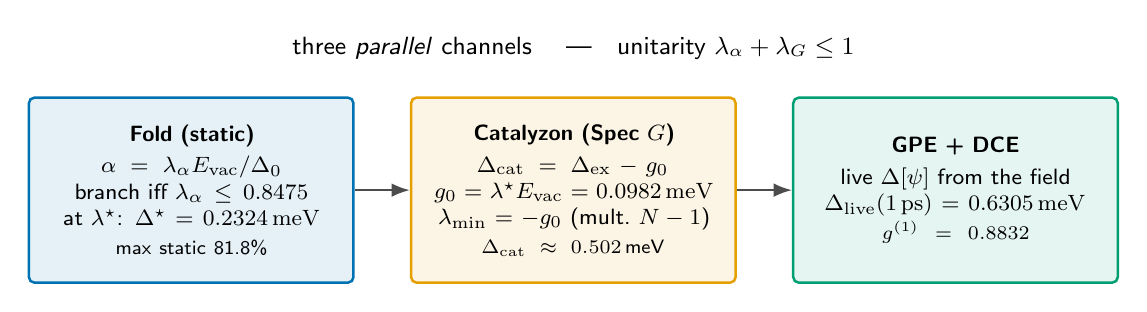
\begin{tikzpicture}[
  font=\sffamily\footnotesize,
  ch/.style={draw=#1, line width=0.9pt, rounded corners=2pt, fill=#1!10,
    align=center, inner sep=6pt, text width=3.7cm, minimum height=2.35cm},
  arr/.style={-{Latex}, thick, gray!60!black}
]
\node[ch=oiBlue] (f) {\textbf{Fold (static)}\\[2pt]
$\alpha=\lambda_\alpha E_{\mathrm{vac}}/\Delta_0$\\
branch iff $\lambda_\alpha\le\lfold$\\
at $\lambda^\star$: $\Delta^\star=\Deltastar$\\[1pt]
{\scriptsize max static \redmax}};
\node[ch=oiOrange, right=0.7cm of f] (c) {\textbf{Catalyzon (Spec $G$)}\\[2pt]
$\Delta_{\mathrm{cat}}=\Delta_{\mathrm{ex}}-g_0$\\
$g_0=\lambda^\star E_{\mathrm{vac}}=\gzerostar$\\
$\lambda_{\min}=-g_0$ (mult.\ $N-1$)\\[1pt]
{\scriptsize $\Delta_{\mathrm{cat}}\approx 0.502$\,meV}};
\node[ch=oiGreen, right=0.7cm of c] (t) {\textbf{GPE + DCE}\\[2pt]
live $\Delta[\psi]$ from the field\\
$\Delta_{\mathrm{live}}(1\,\mathrm{ps})=\Deltaliveone$\\[1pt]
{\scriptsize $g^{(1)}=\goneps$}};
\node[above=0.35cm of c, font=\sffamily\small, align=center]
  {three \emph{parallel} channels \quad---\quad unitarity $\lambda_\alpha+\lambda_G\le 1$};
\draw[arr] (f.east) -- (c.west);
\draw[arr] (c.east) -- (t.west);
\end{tikzpicture}

\caption{\textbf{Parallel catalytic channels.} Static fold, Spec$(G)$ catalyzon, and truncated GPE/DCE dynamics are not additive corrections to one another. The withdrawn stack $35/52/92$ mixed those channels and a $\Delta(t)$ schedule that did not use $\psi$.}
\label{fig:channels}
\end{figure}

\section{Catalyzon and the coupling matrix}
\label{sec:catalyzon}

Five long-wavelength collective modes---Higgs (amplitude), Josephson plasma, flat-band plasmon, hopfion deformation, and Bogoliubov phase---can meet near $\omega_0=2\Delta/\hbar$. Off-diagonal vacuum-mediated couplings assemble a symmetric $N\times N$ matrix $G$ with vanishing diagonal (no on-resonance self-energy at this order) and $\operatorname{Tr} G=0$. The near-resonance Hamiltonian is
\begin{equation}
H=\sum_{i=1}^N\hbar\omega_0 a_i^\dagger a_i+\sum_{i<j}G_{ij}(a_i^\dagger a_j+a_j^\dagger a_i).
\end{equation}

\begin{theorem}[Democratic spectrum]
\label{thm:demo}
For $G=g_0(J_N-I_N)$ one has $\lambda_{\max}=(N-1)g_0$ (multiplicity one; bright) and $\lambda_{\min}=-g_0$ (multiplicity $N-1$; dark/Helmert). The catalyzon gap on this spectrum is $\Delta_{\mathrm{cat}}=\Delta_{\mathrm{ex}}-g_0$. The assignments $\lambda_{\min}=-4g_0$ ($N=5$) and $\lambda_{\min}=-5g_0$ (octahedral folklore) are not eigenvalues of the democratic matrix.
\end{theorem}

\begin{figure}[H]
\centering
% Democratic Spec(G)
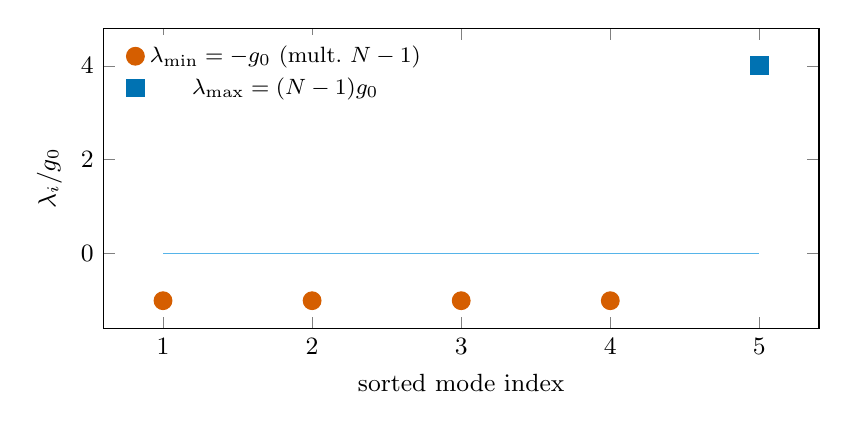
\begin{tikzpicture}
\begin{axis}[
  width=0.88\linewidth,
  height=5.4cm,
  xlabel={sorted mode index},
  ylabel={$\lambda_i/g_0$},
  xtick={1,2,3,4,5},
  ymin=-1.6, ymax=4.8,
  legend style={draw=none, at={(0.02,0.98)}, anchor=north west, font=\footnotesize},
  tick label style={font=\small},
  label style={font=\small},
]
\addplot[only marks, mark=*, mark size=3.2pt, oiVerm]
  coordinates {(1,-1)(2,-1)(3,-1)(4,-1)};
\addlegendentry{$\lambda_{\min}=-g_0$ (mult.\ $N-1$)}
\addplot[only marks, mark=square*, mark size=3.2pt, oiBlue]
  coordinates {(5,4)};
\addlegendentry{$\lambda_{\max}=(N-1)g_0$}
\addplot[oiSky, thin] coordinates {(1,0)(5,0)};
\end{axis}
\end{tikzpicture}

\caption{\textbf{Democratic $\mathrm{Spec}(G)$ for $N=5$.} Dark subspace $\lambda_{\min}=-g_0$ (four-fold) and bright eigenvalue $\lambda_{\max}=4g_0$. Plots or tables quoting $\lambda_{\min}=-4g_0$ are obsolete.}
\label{fig:spec}
\end{figure}

\begin{theorem}[Catalyzon existence]
\label{thm:cat}
Any real symmetric $G\neq 0$ with $\operatorname{Tr} G=0$ has $\lambda_{\min}<0$, hence $\Delta_{\mathrm{cat}}=\Delta_{\mathrm{ex}}+\lambda_{\min}<\Delta_{\mathrm{ex}}$.
\end{theorem}

Theorem~\ref{thm:cat} is model-independent given the trace and symmetry hypotheses. Quantitative matrix elements are not. A program-level construction places five Gaussians on the moir\'e hexagon, convolves with a $K_0(|\mathbf{r}-\mathbf{r}'|/R)$ kernel, and sets $G_{ii}=0$. Democratic $J-I$ is not inserted. The output is Hermitian and traceless, has $\lambda_{\min}<0$, and lies $\sim 7\%$ in relative Frobenius distance from the democratic matrix at the mean off-diagonal; the dark multiplicity is split by the pentagon-in-hexagon geometry rather than exactly $N-1$. Eigenvalues remain in arbitrary units ($g_{0,\mathrm{eff}}\sim 10^{-4}$) until a prefactor is fixed to $g_0=\lambda_G E_{\mathrm{vac}}$. Variation of a torsion action (hypothesis H-TOR1) is not performed. We therefore grade WS $G_{ij}$ as program-computed, not as a derived Einstein--Cartan vertex.

At the phonon resonance, analytic continuation of the one-loop self-energy produces a two-particle threshold $\operatorname{Im}\Sigma^R(\omega)\propto\Theta(\omega-2\Delta/\hbar)\sqrt{\omega-2\Delta/\hbar}$. Using $\Delta^\star$ rather than withdrawn $\Delta_{\mathrm{QVC}}$ shifts the matching wavevector $q^*=2\Delta/(\hbar c_{\mathrm{LA}})$ downward from the historical $0.056$\,nm$^{-1}$; we do not treat that historical number as a lock.

\section{Topological Ginzburg--Landau functional and honest truncation}
\label{sec:tqgl}

The intended low-energy functional is
\begin{equation}
\mathcal{F}[\Psi,\mathbf{a}]=\mathcal{F}_{\mathrm{bulk}}+\mathcal{F}_{\mathrm{CS}}+\mathcal{F}_{\mathrm{Berry}}+\mathcal{F}_{\mathrm{ZPF}}+\mathcal{F}_{\mathrm{Skyrme}},
\label{eq:tqgl}
\end{equation}
with a Mexican-hat bulk, Chern--Simons term at level $k=2N$~\cite{Laughlin1983,Wen1995}, Berry coupling of band curvature to the condensate current~\cite{Xiao2010,Qi2011}, a vacuum shift $\mathcal{F}_{\mathrm{ZPF}}=-\lambda\int A_{\mathrm{ZPF}}|\Psi|^2$, and a Skyrme stabilizer against Derrick collapse~\cite{Faddeev1997,Sutcliffe2007}. Equation~\eqref{eq:tqgl} is the field theory we wish to solve. It is not the equation of motion used in the present numerical program.

The honest truncation is a two-dimensional cubic--quintic Gross--Pitaevskii equation for $\psi(x,y,t)$, with a toroidal potential proportional to the locked $E_{\mathrm{vac}}$ and a coupled ordinary differential equation for a dynamical Casimir amplitude $A(t)$. Chern--Simons, Berry, and Skyrme contributions are omitted from the time stepper. The gap estimator is required to use $\psi$:
\begin{equation}
\Delta_{\mathrm{live}}[\psi]=\Delta_0\sqrt{n_w[\psi]/n_{\mathrm{ref}}},
\label{eq:live}
\end{equation}
where $n_w$ is the ring-weighted mean of $|\psi|^2$ and $n_{\mathrm{ref}}$ is the same average on the initial field. Equation~\eqref{eq:live} does not accept a time argument and cannot reproduce a prescribed schedule $0.600\to 0.389\to 0.200\to 0.032$\,meV.

\begin{figure}[H]
\centering
% Honest TQGL truncation
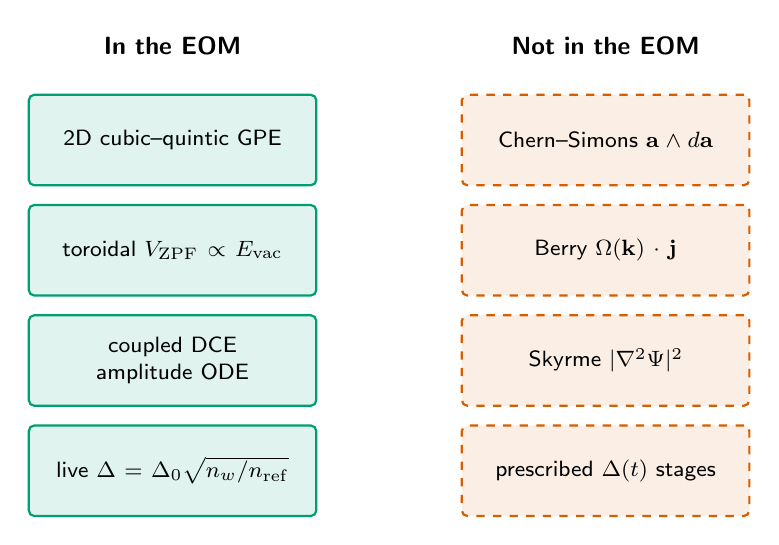
\begin{tikzpicture}[
  font=\sffamily\footnotesize,
  on/.style={draw=oiGreen, line width=0.8pt, fill=oiGreen!12, rounded corners=2pt,
    align=center, inner sep=5pt, text width=3.3cm, minimum height=1.15cm},
  off/.style={draw=oiVerm, line width=0.8pt, fill=oiVerm!10, rounded corners=2pt,
    align=center, inner sep=5pt, text width=3.3cm, minimum height=1.15cm, dashed},
]
\node[font=\sffamily\small\bfseries] (h1) at (0,3.35) {In the EOM};
\node[font=\sffamily\small\bfseries] (h2) at (5.5,3.35) {Not in the EOM};
\node[on] (a) at (0,2.15) {2D cubic--quintic GPE};
\node[on] (b) at (0,0.75) {toroidal $V_{\mathrm{ZPF}}\propto E_{\mathrm{vac}}$};
\node[on] (c) at (0,-0.65) {coupled DCE amplitude ODE};
\node[on] (d) at (0,-2.05) {live $\Delta=\Delta_0\sqrt{n_w/n_{\mathrm{ref}}}$};
\node[off] (e) at (5.5,2.15) {Chern--Simons $\mathbf{a}\wedge d\mathbf{a}$};
\node[off] (f) at (5.5,0.75) {Berry $\Omega(\mathbf{k})\cdot\mathbf{j}$};
\node[off] (g) at (5.5,-0.65) {Skyrme $|\nabla^2\Psi|^2$};
\node[off] (h) at (5.5,-2.05) {prescribed $\Delta(t)$ stages};
\end{tikzpicture}

\caption{\textbf{Truncation of the dynamics.} Left: terms present in the GPE/DCE integrator. Right: topological and Skyrme terms retained only in the parent functional, and the withdrawn prescribed $\Delta(t)$. Live gap extraction is mandatory.}
\label{fig:trunc}
\end{figure}

Linear dynamical Casimir theory predicts exponential growth of the vacuum amplitude under parametric driving~\cite{Uhlmann2004}. The suite actually integrates the first-order amplitude
\begin{equation}
\dot A=\bigl[\Lambda(\Delta)\,\mathcal{L}(\delta\omega/\Gamma)-\Lambda_{\mathrm{loss}}\bigr]A,\qquad
\mathcal{L}(x)=\frac{1}{1+x^2},
\label{eq:dceode}
\end{equation}
with $\Lambda(\Delta)=(m\Delta/2\hbar)\,Q/(2\pi)$ and $\Lambda_{\mathrm{loss}}$ equal to the cavity linewidth at $\Delta^\star$. On the $1$\,ps window, $\Delta$ in Eq.~\eqref{eq:dceode} is $\Delta_{\mathrm{live}}[\psi]$. On an $80$\,ps window, $\Delta$ is slaved to the physical fold branch $\Delta(A)$, justified by $\Gamma_{\mathrm{cav}}^{-1}$ of tens of picoseconds. Chern--Simons, Berry, and Skyrme terms remain absent from both windows. Lindblad dissipation is not included.

The coupled split-step run ($128\times 128$ on a $200$\,nm box, $\mathrm{d}t=2$\,fs, hopfion initial data with $10\%$ core depletion, $Q_H\theta$ phase, and $3\%$ noise) does \emph{not} collapse. The live gap starts at $\Delta_{\mathrm{live}}(0)=0.6000$\,meV by construction of $n_{\mathrm{ref}}$ and ends at $\Delta_{\mathrm{live}}(1\,\mathrm{ps})=\Deltaliveone$. The minimum on the trajectory is $0.6000$\,meV, so the live gap never crosses $\Delta_c$. Coherence is $g^{(1)}(1\,\mathrm{ps})=\goneps$, and $A(1\,\mathrm{ps})/A_c^{\mathrm{fold}}=\AoneAc$, with relative $\|\psi\|$ drift $1.30\times 10^{-14}$. The withdrawn $0.032$\,meV and $92\%$ figures are not outputs of this integrator.

Fold-slaved DCE over $80$\,ps saturates without folding out. The resonant case ($L(0)=1$) reaches $A^*/A_c^{\mathrm{fold}}=\AresAc$ with $\Delta_{\mathrm{ss}}=\Deltassres$. The detuned case ($L(0)=0.200$) reaches $\AdetAc$ with $\Delta_{\mathrm{ss}}=\Deltassdet$. Those ratios are computed; they are not the withdrawn drive factor $E_{\mathrm{vac}}/0.244\approx 0.527$ and they are not a fitted $0.52$.

Schwinger and Berry diagnostics are \emph{not} in the equation of motion. Identifying $g_0=\lambda^\star E_{\mathrm{vac}}=\gzerostar$ gives $|\lambda_{\min}|=\gzerostar$, $E_{\mathrm{pair}}=\Epair$ (not $0.172$\,meV), and a crossover $T^*=\Tstar$. A GOE/GUE Monte Carlo probe of $\lambda_{\min}$ yields mean ratio $R=\BerryR$, not a forced $1.43$ Berry enhancement.

\begin{figure}[H]
\centering
% Coupled GPE 1 ps: live gap from psi (not a schedule)
\begin{tikzpicture}
\begin{axis}[
  width=0.92\linewidth,
  height=5.6cm,
  xlabel={$t$ (ps)},
  ylabel={$\Delta_{\mathrm{live}}[\psi]$ (meV)},
  xmin=0, xmax=1.02,
  ymin=0.08, ymax=0.72,
  legend style={draw=none, at={(0.02,0.98)}, anchor=north west, font=\footnotesize},
  tick label style={font=\small},
  label style={font=\small},
]
\addplot[oiBlue, thick]
  table[col sep=comma, x=t_ps, y=Delta_live_meV] {data/coupled_timeseries_plot.csv};
\addlegendentry{$\Delta_{\mathrm{live}}$}
\addplot[oiOrange, densely dashed]
  table[col sep=comma, x=t_ps, y=Delta_fold_of_A_meV] {data/coupled_timeseries_plot.csv};
\addlegendentry{fold $\Delta(A)$}
\addplot[oiGreen, densely dotted] coordinates {(0,0.600) (1.02,0.600)};
\addlegendentry{$\Delta_0$}
\addplot[oiVerm, densely dotted] coordinates {(0,0.1091) (1.02,0.1091)};
\addlegendentry{$\Delta_c$}
\end{axis}
\end{tikzpicture}

\caption{\textbf{Live gap on the truncated GPE.} $\Delta_{\mathrm{live}}[\psi]$ over $1$\,ps (solid) compared with the instantaneous fold branch $\Delta(A)$ (dashed). Horizontal guides mark $\Delta_0$ and $\Delta_c$. The live gap rises to $\Deltaliveone$ and never falls below $\Delta_c$. Data: \texttt{coupled\_timeseries.csv}.}
\label{fig:live}
\end{figure}

\begin{figure}[H]
\centering
% Coupled GPE: coherence and DCE amplitude
\begin{tikzpicture}
\begin{axis}[
  width=0.92\linewidth,
  height=5.4cm,
  xlabel={$t$ (ps)},
  ylabel={$g^{(1)}$,\ $A/A_c^{\mathrm{fold}}$},
  xmin=0, xmax=1.02,
  ymin=0.82, ymax=1.02,
  legend style={draw=none, at={(0.02,0.02)}, anchor=south west, font=\footnotesize},
  tick label style={font=\small},
  label style={font=\small},
]
\addplot[oiPurple, thick]
  table[col sep=comma, x=t_ps, y=g1] {data/coupled_timeseries_plot.csv};
\addlegendentry{$g^{(1)}$}
\addplot[oiBlue, thick, dashed]
  table[col sep=comma, x=t_ps, y expr={\thisrow{A_um_inv}/1.558248}] {data/coupled_timeseries_plot.csv};
\addlegendentry{$A/A_c^{\mathrm{fold}}$}
\end{axis}
\end{tikzpicture}

\caption{\textbf{Coherence and vacuum amplitude.} First-order coherence $g^{(1)}$ and $A/A_c^{\mathrm{fold}}$ on the same $1$\,ps window. Final values $g^{(1)}=\goneps$ and $A/A_c^{\mathrm{fold}}=\AoneAc$.}
\label{fig:g1A}
\end{figure}

\section{Hopfions and fractional Hall charge}
\label{sec:hopf}

Hopfions are maps $\hat{\mathbf{n}}:\mathbb{R}^3\to S^2$ classified by the Hopf invariant, the linking number of preimages~\cite{Faddeev1997,Sutcliffe2007,Ackerman2017,Kent2021}. In an $N$-layer \TEVC{} the configuration space carries a $\mathbb{Z}_N$ identification, and the effective topology is the lens space $L(N,1)=S^3/\mathbb{Z}_N$. The integral homology is $H_1\cong\mathbb{Z}_N$ and $H_2(L(N,1);\mathbb{Z})=0$. Any argument that fractionalizes $Q_H$ by integrating curvature over a fundamental $2$-cycle is therefore invalid.

\begin{theorem}[Fractional charge from Chern--Simons/linking]
\label{thm:qh}
Flat $U(1)$ connections on $L(N,1)$ are labeled by holonomy $k\in\{0,\ldots,N-1\}$. Their Chern--Simons invariants and the rational linking form on $H_1$ satisfy~\cite{Witten1989,Jeffrey1992}
\begin{equation}
\mathrm{CS}[A_k]=\frac{k^2}{N}\pmod{\mathbb{Z}},\qquad
\mathrm{lk}([\gamma],[\gamma])=\frac1N\pmod 1,
\end{equation}
and the associated fractional Hall charge is $Q_H=1/N$. For five-layer \MATBG{}, $Q_H=1/5$.
\end{theorem}

Each hopfion nucleation event then changes the Hall conductance by
\begin{equation}
\delta\sigma_{xy}=\frac{e^2}{2Nh}=\frac{Q_H e^2}{2h}.
\end{equation}
For $N=5$ this is $\delta\sigma_{xy}\approx 7.75\times 10^{-6}$\,S. The interpretation of $Q_H=1/N$ as the shared invariant between \QVC{} fractionalization and hopfion-spacetime ideation is hypothesis H-SHARE1; the CS/linking identities themselves are locked.

\begin{figure}[H]
\centering
% Lens space L(5,1) schematic (2D, CS/linking)
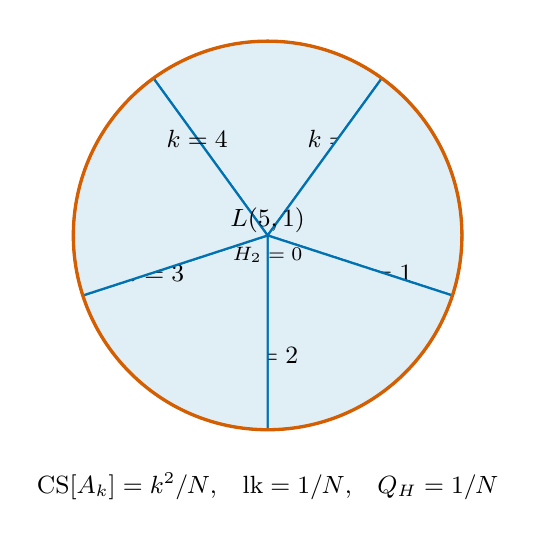
\begin{tikzpicture}[scale=1.05]
\foreach \k in {0,...,4}{
  \pgfmathsetmacro{\ang}{90-72*\k}
  \pgfmathsetmacro{\angb}{\ang-36}
  \fill[oiBlue!12, draw=oiBlue, thick]
    (0,0) -- ({\ang+36}:2.35) arc ({\ang+36}:{\ang-36}:2.35) -- cycle;
  \node[font=\small] at ({\angb}:1.45) {$k=\k$};
}
\draw[oiVerm, very thick] (0,0) circle (2.35);
\node[font=\small, align=center] at (0,0) {$L(5,1)$\\[1pt]{\scriptsize $H_2=0$}};
\node[font=\small, below] at (0,-2.75) {$\mathrm{CS}[A_k]=k^2/N$,\quad $\mathrm{lk}=1/N$,\quad $Q_H=1/N$};
\end{tikzpicture}

\caption{\textbf{Lens space $L(5,1)$.} Five holonomy sectors with $\mathrm{CS}[A_k]=k^2/N$. Because $H_2=0$, fractionalization is read from Chern--Simons and linking on $H_1$, not from a surface integral of Berry curvature.}
\label{fig:lens}
\end{figure}

Analogue acoustic geometry~\cite{Unruh1981,Barcelo2011,Volovik2003,Steinhauer2016} can match an Unruh--Visser temperature to a Schwinger crossover by fixing $R_{\mathrm{WS}}=\hbar c_s/(\pi k_B T^*)$. That matching is not a bulk/boundary duality (hypothesis H-HAWK1). A suite diagnostic that is \emph{not} in the GPE, using $E_{\mathrm{pair}}=\Epair$ from $g_0=\lambda^\star E_{\mathrm{vac}}$, gives $T^*=\Tstar$, replacing the historical $285$\,mK that used withdrawn $g_0$.

\section{Experimental signatures}
\label{sec:experiments}

Hall transport as a function of twist, pressure, or displacement field should exhibit a staircase with step $\delta\sigma_{xy}=e^2/(2Nh)$ if hopfion nucleation is the charge-carrying process. The step height measures $Q_H$ independently of the vacuum meV freeze.

A circularly polarized drive at $\omega_L=2\Delta/\hbar$, with $\Delta$ taken from the working static gap $\Delta^\star$ rather than from withdrawn $\Delta_{\mathrm{QVC}}$, is predicted to produce three coincident responses~\cite{Engels2007,Vudragovic2019}: Faraday-wave sidebands and discrete nucleation events scaling as the square of the drive (Mathieu instability); Hall steps in lockstep with nucleation; and superlinear pair luminescence once the first instability tongue is crossed~\cite{Heisenberg1936,Schwinger1951,Dunne2009}. All three should collapse when $\omega_L$ is detuned from $2\Delta/\hbar$. This triple coincidence is a vacuum-catalysis test that does not require accepting any particular historical percentage.

Cavity-QED experiments already demonstrate vacuum-field control of quantum Hall phases in split-ring geometries~\cite{Enkner2025,Jiang2025,Bretscher2026}. The \TEVC{} proposal is that the moir\'e stack is an \emph{intrinsic} cavity. Layer-number dependence of the tunneling gap at fixed twist is a qualitative prediction of self-cavitation; we do not recycle numerical finesse factors that were tied to $A\xi=0.296$.

External resonators hybridize with the bright eigenvalue of $G$, producing catalyzon-polaritons. Avoided crossings should track $\lambda_{\max}=(N-1)g_0$, not a spurious $-4g_0$ dark shift.

\section{Epistemic status}
\label{sec:status}

Figure~\ref{fig:status} is the intended reading order of this paper. Proven algebra (fold, democratic spectrum, CS/linking, the form of the bridge) does not automatically license a laboratory meV. Computed $E_{\mathrm{vac}}=\Evac$ is the output of a frozen-working triple and replaces $0.244$\,meV inside that triple only. Participation $\lambda^\star$ is a derived operating choice, not an overlap integral extracted from $\psi$. Wigner--Seitz $G_{ij}$ is a program computation. Vortex RG, torsion vertices, and \TDVT{} spacetime ontology remain conjectural and are excluded from the abstract as derived claims.

\begin{figure}[H]
\centering
% Status of results
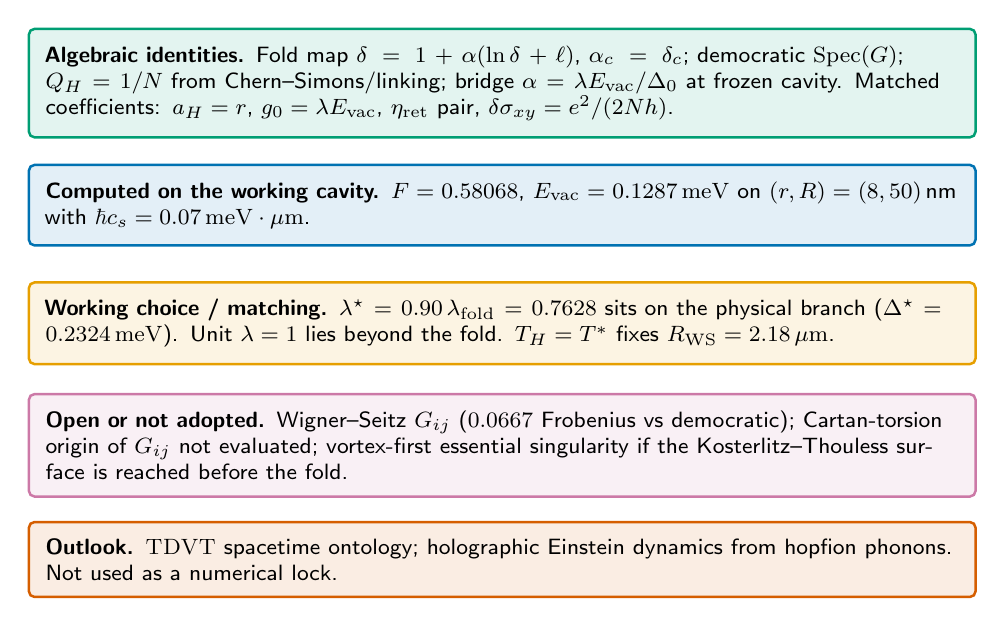
\begin{tikzpicture}[
  font=\sffamily\footnotesize,
  ly/.style={draw=#1, line width=0.9pt, fill=#1!11, rounded corners=2pt,
    align=left, inner sep=6pt, text width=11.6cm},
]
\node[ly=oiGreen] (p) at (0,3.1) {\textbf{Algebraic identities.} Fold map $\delta=1+\alpha(\ln\delta+\ell)$, $\alpha_c=\delta_c$; democratic $\mathrm{Spec}(G)$; $Q_H=1/N$ from Chern--Simons/linking; bridge $\alpha=\lambda E_{\mathrm{vac}}/\Delta_0$ at frozen cavity. Matched coefficients: $a_H=r$, $g_0=\lambda E_{\mathrm{vac}}$, $\eta_{\mathrm{ret}}$ pair, $\delta\sigma_{xy}=e^2/(2Nh)$.};
\node[ly=oiBlue] (c) at (0,1.55) {\textbf{Computed on the working cavity.} $F=\Flock$, $E_{\mathrm{vac}}=\Evac$ on $(r,R)=(8,50)$\,nm with $\hbar c_s=\hbarcs$.};
\node[ly=oiOrange] (w) at (0,0.05) {\textbf{Working choice / matching.} $\lambda^\star=0.90\,\lambda_{\mathrm{fold}}=\lstar$ sits on the physical branch ($\Delta^\star=\Deltastar$). Unit $\lambda=1$ lies beyond the fold. $T_H=T^*$ fixes $R_{\mathrm{WS}}=\RwsMatch$.};
\node[ly=oiPurple] (g) at (0,-1.5) {\textbf{Open or not adopted.} Wigner--Seitz $G_{ij}$ ($\relfroG$ Frobenius vs democratic); Cartan-torsion origin of $G_{ij}$ not evaluated; vortex-first essential singularity if the Kosterlitz--Thouless surface is reached before the fold.};
\node[ly=oiVerm] (x) at (0,-2.95) {\textbf{Outlook.} \TDVT{} spacetime ontology; holographic Einstein dynamics from hopfion phonons. Not used as a numerical lock.};
\end{tikzpicture}

\caption{\textbf{Proven, computed, working, program, and withdrawn.} Status tags are not interchangeable. In particular, computed $E_{\mathrm{vac}}$ is not a measured gap, and L3 spacetime is not an output of the fold theorem.}
\label{fig:status}
\end{figure}

Table~\ref{tab:locks} collects the Option~A* numbers used in the text.

\begin{table}[H]
\centering
\caption{Locked and working quantities for Option~A* (fat torus, Tier-C, frozen-cavity bridge). Status: P~=~proven algebra; C~=~computed on the freeze; W~=~working choice; Pr~=~program.}
\label{tab:locks}
\begin{tabular}{@{}lllc@{}}
\toprule
Quantity & Value & Meaning & Status \\
\midrule
$(r,R)$ & $(8,50)$\,nm & fat-torus cavity & W \\
$\hbar c_s$ & $\hbarcs$ & platform scale & W \\
$F(x)$ & $\Flock$ & Bessel sum at $x\approx 1.005$ & C \\
$E_{\mathrm{vac}}$ & $\Evac$ & Tier-C energy (replaces $0.244$\,meV) & C \\
$\ell(r)$ & $\elllock$ & frozen-cavity log ($\ell_{\mathrm{Corr}}=\ellcorr$) & P \\
$\alpha_c=\delta_c$ & $\alphac$ & fold critical point & P \\
$\Delta_0$ & $\Deltaex$ & bare exchange $2J$ & input \\
$\Delta_c$ & $\Deltac$ & gap at the fold & P \\
max static reduction & $\redmax$ & $1-\delta_c$ & P \\
$\lambda_{\mathrm{fold}}$ & $\lfold$ & unitarity bound of the fold & C \\
$\lambda^\star$ & $\lstar$ & $0.90\,\lambda_{\mathrm{fold}}$ & W \\
$\Delta^\star$ & $\Deltastar$ & physical gap at $\lambda^\star$ (\redstar) & C \\
$\lambda_{\min}$ & $-g_0$ ($\times N-1$) & democratic dark subspace & P \\
$g_0=\lambda^\star E_{\mathrm{vac}}$ & $\gzerostar$ & suite catalyzon scale & W \\
$\Delta_{\mathrm{live}}(1\,\mathrm{ps})$ & $\Deltaliveone$ & GPE live gap (rose) & Pr \\
$g^{(1)}(1\,\mathrm{ps})$ & $\goneps$ & coherence & Pr \\
$A^*/A_c^{\mathrm{fold}}$ (res./det.) & $\AresAc$ / $\AdetAc$ & DCE saturation (not $0.52$) & Pr \\
$T^*$ & $\Tstar$ & Schwinger diagnostic (not in EOM) & Pr \\
$Q_H$ & $1/N$ & CS/linking on $L(N,1)$ & P \\
$\eta_{\mathrm{ret}}$ & $\etaret$ & causal-propagator retardation & W \\
WS rel.\ Frobenius & $\sim 7\%$ & $G_{ij}$ vs democratic & Pr \\
\bottomrule
\end{tabular}
\end{table}

\section{Discussion}
\label{sec:discussion}

The central change relative to the v3 preprint is not rhetorical. It is the replacement of an audit-failed Casimir number and a prescribed dynamical schedule by a freeze that can be stated in one sentence: Tier-C form, fat torus, package $\hbar c_s$, derived bridge, fold theorem. That sentence implies fold-out at $\lambda=1$ and a maximum static reduction of $\redmax$. It also implies that three historical percentages cannot be stacked.

Several limitations are structural. First, $\hbar c_s=\hbarcs$ is a package scale; SI conversion and optical versus phononic identification remain open at $\mathcal{O}(1)$. Second, $\lambda^\star$ is not measured. Third, the GPE truncation omits Chern--Simons, Berry, and Skyrme terms, so the $1$\,ps live-gap rise to $\Deltaliveone$ is not a topological Hall simulation. Fourth, Wigner--Seitz $G_{ij}$ still lacks a torsion derivation (H-TOR1). Fifth, retardation $\eta_{\mathrm{ret}}\approx\etaret$ uses a coherence length that is not identical to the freeze $R$. Sixth, analogue Hawking matching is not a holographic dictionary~\cite{Hartnoll2018,Maldacena1999}; we do not derive Einstein equations from hopfion phonons. The $1$\,ps window also omits Lindblad dissipation.

Cavity-QED and vacuumronics~\cite{Enkner2025,Jiang2025,Bretscher2026} provide the closest experimental language: engineered vacuum fluctuations as a control knob. The \TEVC{} claim is that moir\'e geometry already supplies such a knob, with the fold map as the condensed-matter readout. Confirmation would be a materials route to barrier engineering. Extensions to Coulomb barriers in fusion plasmas remain speculative and are not quantified here; no meV-to-MeV extrapolation is offered, and no net energy is taken from the vacuum.

\section{Conclusions}
\label{sec:conclusions}

Quantum Vacuum Catalyzation is a catalytic, energy-conserving coupling of zero-point modes to a topochiral excitonic condensate. On Option~A* the toroidal vacuum energy is $E_{\mathrm{vac}}=\Evac$ with $F=\Flock$, the gap map is a fold at $\alpha_c=\alphac$, and unit participation is past that fold. Working static physics sits at $\lambda^\star=\lstar$ with $\Delta^\star=\Deltastar$ ($\redstar$), while the deepest physical static reduction is $\redmax$. Democratic catalyzon physics is parallel, with $\lambda_{\min}=-g_0$ (multiplicity $N-1$). Truncated GPE dynamics with a live gap from $\psi$ give $\Delta_{\mathrm{live}}(1\,\mathrm{ps})=\Deltaliveone$ (an increase, not a $92\%$ collapse) and $g^{(1)}=\goneps$; fold-slaved DCE saturates at $A^*/A_c^{\mathrm{fold}}=\AresAc$ (resonant) and $\AdetAc$ (detuned). Fractional Hall charge $Q_H=1/N$ is a Chern--Simons/linking identity. Spacetime ontology is not derived. The withdrawn quartet $0.244$\,meV, $0.389$\,meV, $0.032$\,meV, and $92\%$ is retained only as an audit trail in Appendix~\ref{app:folklore}.

\section*{Acknowledgments}
The author thanks computational resources used to freeze the Option~A* triple and to solve the fold map. No funding to declare.

\appendix
\section{Fold critical table}
\label{app:fold}
The dimensionless map $\delta=1+\alpha(\ln\delta+\ell)$ with frozen-cavity $\ell=\elllock$ (Corrections $\ell=\ellcorr$) has critical values $\delta_c=\alpha_c=\alphac$, $\Delta_0=\Deltaex$ (input), and $\Delta_c=\Deltac$. Near-fold scaling is $\delta-\delta_c\sim\pm\sqrt{\alpha_c-\alpha}$. Tree-level running healing produces $\ell_{\mathrm{tree}}\approx-0.11593$ and is not the freeze. BKT language remains contingent on vortex RG. Data: \texttt{data/fold\_phys.dat}, \texttt{data/fold\_unst.dat}.

\section{Withdrawn folklore}
\label{app:folklore}
The following quantities are \emph{not} physical outputs of Option~A* and must not be quoted as results. $F=0.596$ is replaced by $\Flock$. $E_{\mathrm{Cas}}=0.244$\,meV is not reproduced by the old Casimir formula on $(8,50)$\,nm (that formula gives $2.527$\,meV) and is replaced by $E_{\mathrm{vac}}=\Evac$ under Tier~C. $A\xi=0.296$ is replaced by $AR\approx 0.0919$. $\Delta_{\mathrm{QVC}}=0.389$\,meV was a unit-participation static root of an inconsistent energy; at $\lambda=1$ the present bridge is fold-out, and $0.389$\,meV would require $E\approx 0.065$\,meV or $\lambda\approx 0.508$. The label $35\%$ is that inconsistent static reduction. The label $52\%$ mixed $(\Delta_{\mathrm{QVC}}-0.1)/\Delta_{\mathrm{ex}}$. The label $92\%$ is $(0.389-0.032)/0.389$; versus $\Delta_0$ the same $0.032$\,meV is a $94.7\%$ drop, and $\delta=0.032/0.6$ lies below $\delta_c$. Jacobi $\vartheta_3\equiv F$ is withdrawn. Democratic $\lambda_{\min}=-4g_0$ is withdrawn. Working $g_0=0.21$\,meV is withdrawn as a vacuum scale.

\section{Data and figure provenance}
\label{app:data}
Fold and $\lambda$ scans are generated from \texttt{qvc.gap\_fold} and \texttt{qvc.gap\_reduction} in \QVC{}Compute. $F(x)$ is the Bessel sum in \texttt{qvc.vacuum\_freeze}. Matplotlib freeze figures (fold operating point, $F(x)$, $G_{ij}$ heatmap and spectrum, $\lambda$ partition) are copied from the freeze suite into \texttt{figures/} for archival comparison; publication line art in the main text is TikZ/PGFPlots. The archival PNG of a $0.244$\,meV drive rescaling is a diagnostic only and is not displayed above.

\bibliographystyle{unsrt}
\bibliography{qvc_refs}

\end{document}
